\documentclass[]{article}
\usepackage{amsmath,amsfonts,amssymb,fancyhdr, enumerate, graphicx}
\usepackage[bottom]{footmisc}
\usepackage{setspace}
\usepackage{cite}
\doublespacing
\graphicspath{ {/LaTeX Images} }

\pagestyle{fancy}  
\oddsidemargin 1cm
\hoffset-1cm
\voffset-0.5cm
\topmargin-1.4cm
\textheight 24cm \textwidth 16.5cm \parindent 0.5cm

\begin{document}
\section{Methods}
        \subsection{Introduction}
        All numerical calculations were carried out with \textit{R} \cite{R}. The third party packages \textit{deSolve} \cite{deSolve}, \textit{phaseR} \cite{phaseR} and \textit{ggplot2} \cite {ggplot} were used for modelling the equations, finding nullclines, constructing phase portraits and plotting the behaviour for each system. The diagrams have been constructed in order to adhere to the graphical notation for biological networks as proposed by Kitano in \cite{standardNotation}.
	            
        \subsection{A Single Gene System} 
        The simplest case to consider when modelling the interactions of genes and protein is the interaction of a single gene with its protein. There are three possible scenarios to consider in this case. The protein can feed back positively into its transcription (Figure \ref{singlePositive}), it can feed back negatively or it can have no affect its transcription at all. The last case is of no real interest to us and won't be looked at further. The first two cases, do however give rise to interesting dynamical systems and will be the focus of this section. 
        	     
        \begin{figure}[h]
        \centering
        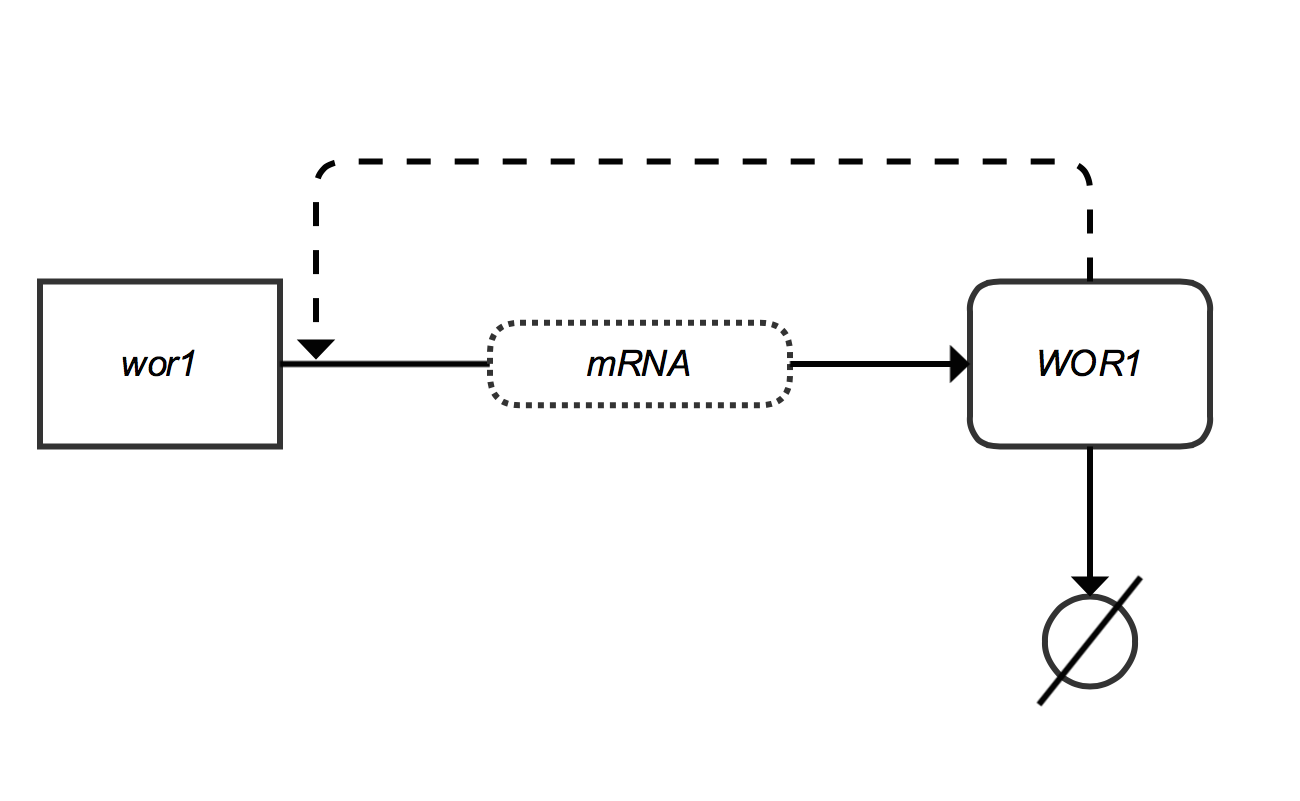
\includegraphics[width=0.6\textwidth]{./figures/singlePositive.png}
        \caption{Positive feedback system of the \textit{wor1} gene's feedback with the WOR1 protein, including mRNA and degradation of the protein.}
        \label{singlePositive}
        \end{figure}            

        \begin{figure}[h]
        \centering
        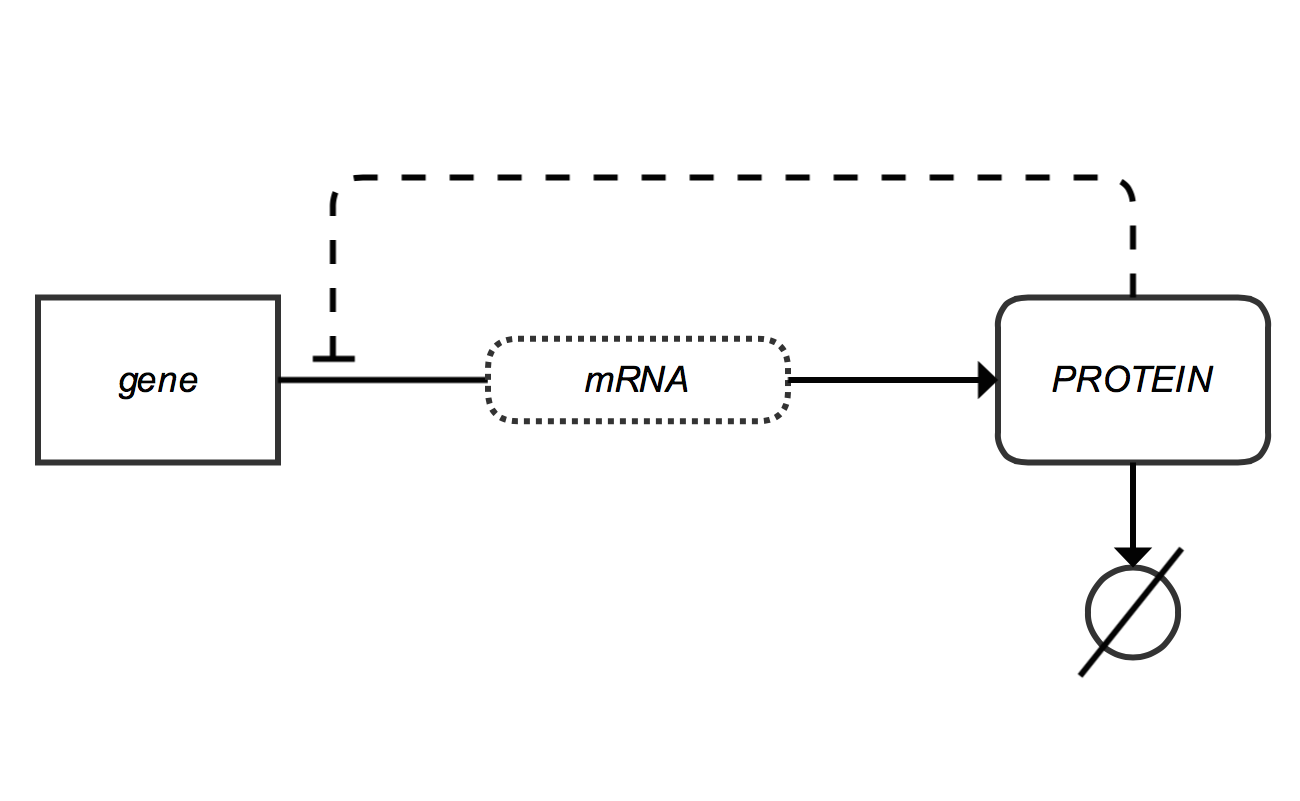
\includegraphics[width=0.6\textwidth]{./figures/singleNegative.png}
        \caption{Negative feedback system of a gene with a protein including mRNA and degradation of the protein.}
        \label{singleNegative}
        \end{figure}
        
        %@Steph do we need to change ligand%
        The approach taken to constructing a system of equations for a positive and negative feedback dynamical system was inspired by the approach of de Jong in \cite{slides}, it includes mRNA, protein and degradation. Hills equation is used to model the fraction of possible binding sites on the receptor ('promoter' region of wor1 gene on DNA strands) that are occupied by a ligand (wor1 protein)... ignoring any interruptions of binding sites due to other molecules in the cell.
        
            \subsubsection{Positive Feedback} 
            Using this approach the positive feedback system depicted in Figure \ref{singlePositive} can be mathematically described by the following equations.
            
            \begin{align*}
                \frac{dx_1}{dt} &= \kappa_1 h(x_2) - \gamma_1 x_1 \\
                \frac{dx_2}{dt} &= \kappa_2x_1- \gamma_2 x_2\\
                \text{The variables are denoted as:}&\\
                x_1 &= \text{Concentration of mRNA}\\
                x_2 &= \text{Concentration of Protein}\\
                \kappa_1, \kappa_2 &= \text{Production Rate of mRNA and Protein respectively}\\
                \gamma_1, \gamma_2 &= \text{Degredation Rate of mRNA and Protein respectively}\\
                h(x) &= \frac{x^n}{k^n+x^n} \text{where $k$ describes a threshold concentration and $n$ a strength}
            \end{align*}
            
            One of these single gene positive feedback system as described above exists in Candida Albicans, for the sake of relevance we'll be discussing the above system as it pertains to this specific system where the gene is \textit{wor1} and the protein is WOR1. 
            
            In order to investigate the system further the nullclines and phase portrait are plotted in Figure \ref{stabilitySinglePositive}. We can see from these that there are three stationary points in this system. The middle stationary point around $(1,1)$ is not stable and of not much practical interest as even infinitesimally small perturbations will cause it to tend towards one of the other stationary points of which are both stable. It can be concluded from this that the system is bi-stable as there are exactly two stability points. Taking this one step further the behaviour of the protein around these stability points can be investigated to get a sense of the difference in physical state of the system being at either of the stability points. 
            
             \begin{figure}[h]
            \centering
            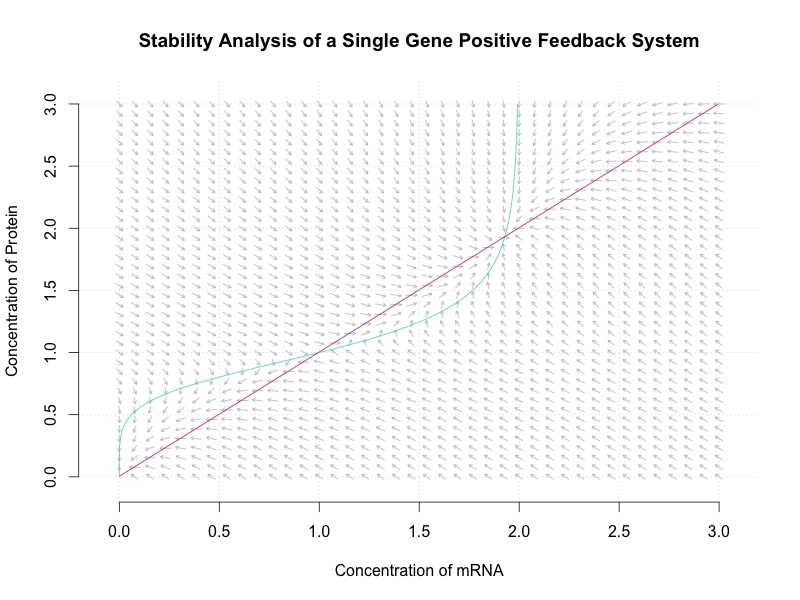
\includegraphics[width=0.6\textwidth]{./figures/stabilitySinglePositive.jpeg}
            \caption{The stability of stationary point present in a single gene positive feedback system. The red line represents the nullcline for the protein and blue the nullcline of mRNA. The arrows represent the direction of change for the system at a given state.}
            \label{stabilitySinglePositive}
            \end{figure}
            
                    
             \begin{figure}[h]
            \centering
            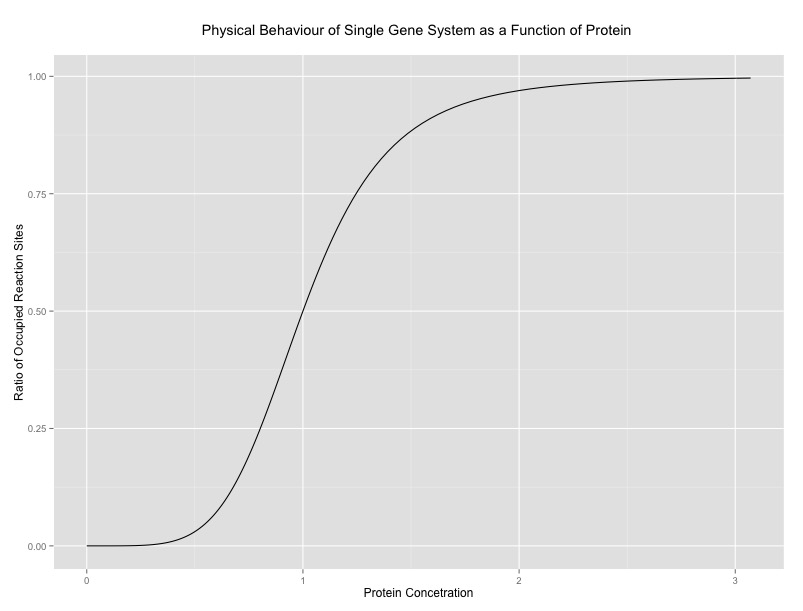
\includegraphics[width=0.6\textwidth]{./figures/singlePositiveHill.jpeg}
            \caption{Compares the fraction of occupiable receptor sites on the protein that are currently occupied against the concentration of protein.}
            \label{singlePositiveHill}
            \end{figure}
    
            The fraction of occupiable binding sites on the receptor was modelled against the concentration of protein in Figure \ref{singlePositiveHill}. This shows that as the concentration of protein increases the ratio of occupied receptor sites increases until all sites are occupied. We can think of this as a state where %%@Steph what does having a heap of protein mean? 
            White is dominant and Opaque is subdued %%This is completele ramble DO NOT INCLUDE IN FINAL WITHOUT CHECKING
            
            \subsubsection{Negative Feedback} 
            The same approach as used in analysing the positive feedback system was applied to modelling the negative feedback system. The only difference in the set of equations that describe the system is a modification to the Hill equation. Instead of the hill equation being $h(x) = \frac{x^n}{k^n + x^n}$ we use $h(x) = \frac{k^n}{k^n+x^n}$. This is a small modification with quite a drastic impact. Modelling the nullclines and phase portrait to investigate the behaviour of the system around its stability points in Figure \ref{stabilitySingleNegative} we can see that the negative feedback system has only one stationary point which is in turn its only stability point. It appears that the negative feedback system of a single gene is incapable of producing a bistable or multi stable state.
            
            \begin{figure}[h]
            \centering
            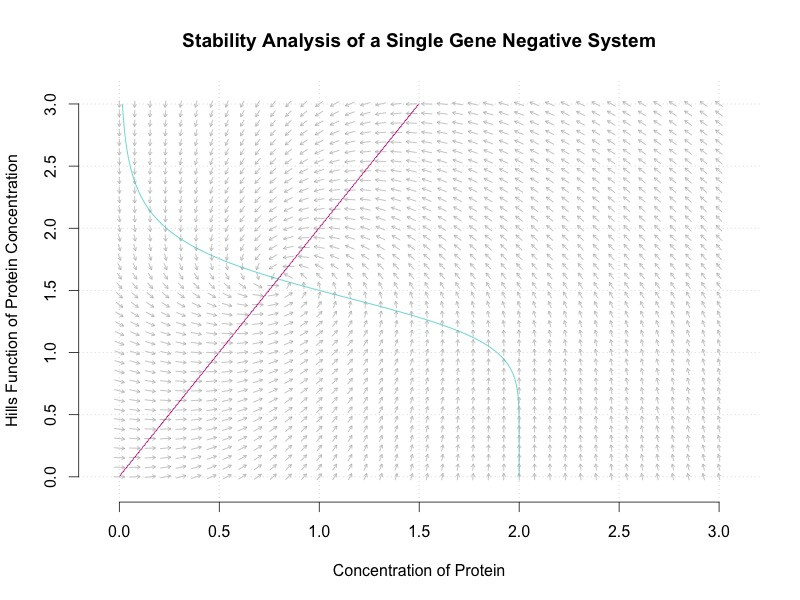
\includegraphics[width=0.6\textwidth]{./figures/stabilitySingleNegative.jpeg}
            \caption{The stability of stationary point present in a single gene negative feedback system. The red line represents the nullcline for the protein and blue the nullcline of mRNA. The arrows represent the direction of change for the system at a given state.}
            \label{stabilitySingleNegative}
            \end{figure}
            
\pagebreak
        \subsection{Multiple Gene Systems}
        A vast number of multiple gene feedback loops are possible, sadly most of these systems are out of the scope of this paper. %Tears, lots of tears. 
        The two that will be investigated are mutual positive feedback between two genes and mutual negative feedback between two genes. A different approach to modelling these will be adopted as compared two the single gene cases. In order to keep things relatively manageable the impact of mRNA will be neglected and only the concentration of protein in each system will be looked at, this is the simplified approach to this problem adopted by de Jong in \cite{multiGene}. 

        \begin{figure}[h]
        \centering
        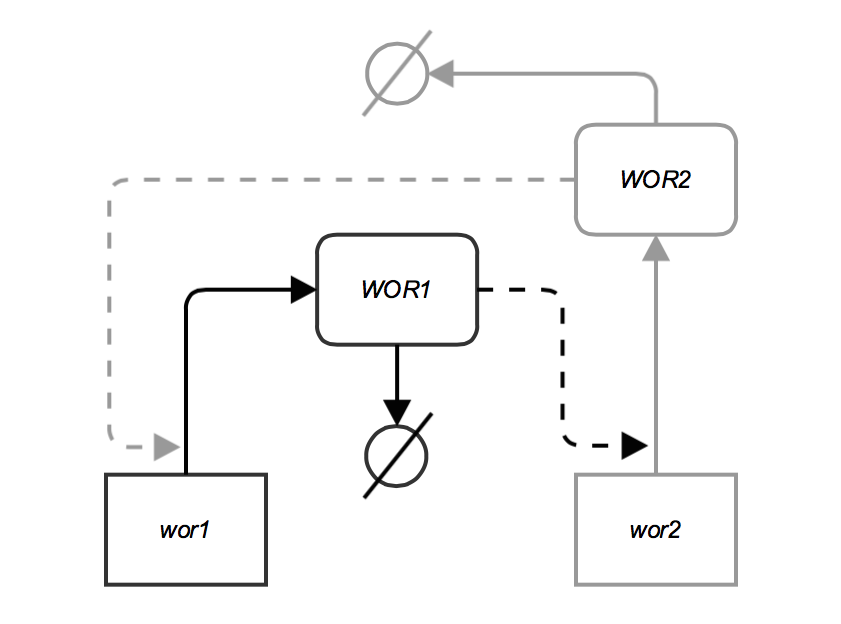
\includegraphics[width=0.6\textwidth]{./figures/doublePositive.png}
        \caption{Positive feedback system of the \textit{wor1} gene and the \textit{work2} gene whereby WOR1 promotes WOR2 and WOR 2 promotes WOR1}
        \label{doublePositive}
        \end{figure}            
    
        \begin{figure}[h]
        \centering
        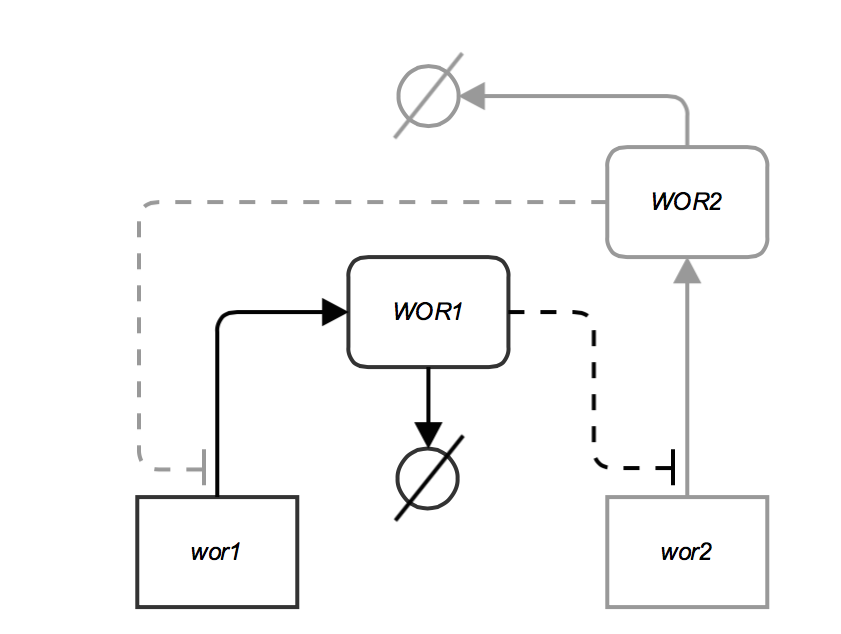
\includegraphics[width=0.6\textwidth]{./figures/doubleNegative.png}
        \caption{Negative feedback system of two genes where the protein mutually inhibit each other.}
        \label{doubleNegative}
        \end{figure}
                 
            \subsubsection{Positive Feedback}
            A network of 2 genes with mutual positive feedback also exits in the Candida Albicans cell between the \textit{wor1} \& \textit{wor2} genes, this is the system as depicted in Figure \ref{doublePositive}. The equations describing this system are given below.
            
            \begin{align*}
                \frac{dx_1}{dt} &= \kappa_1 h(x_2) - \gamma_1 x_1 \\
                \frac{dx_2}{dt} &= \kappa_2 h(x_1) - \gamma_2 x_2 \\
                \text{The variables are denoted as:}&\\
                x_1 &= \text{Concentration of WOR1}\\
                x_2 &= \text{Concentration of WOR2}\\
                \kappa_1, \kappa_2 &= \text{Production Rate of WOR1 and WOR2 respectively}\\
                \gamma_1, \gamma_2 &= \text{Degredation Rate of WOR1 and WOR2 respectively}\\
                h(x) &= \frac{x^n}{k^n+x^n} \text{where $k$ describes a threshold concentration and $n$ a strength}
            \end{align*}
            
            Again, the nullclines and phase portrait are plotted to investigate the behaviour around the stability points. This can be seen in Figure \ref{stabilityDoublePositive}. This system behaves somewhat similar to the single gene positive feedbacks system, similarly it has three stationary points, two of which are stable and one of  which is unstable. This makes sense when considering the behaviour of the general system %% Bullshiting need to elaborate
            
            \begin{figure}[h]
            \centering
            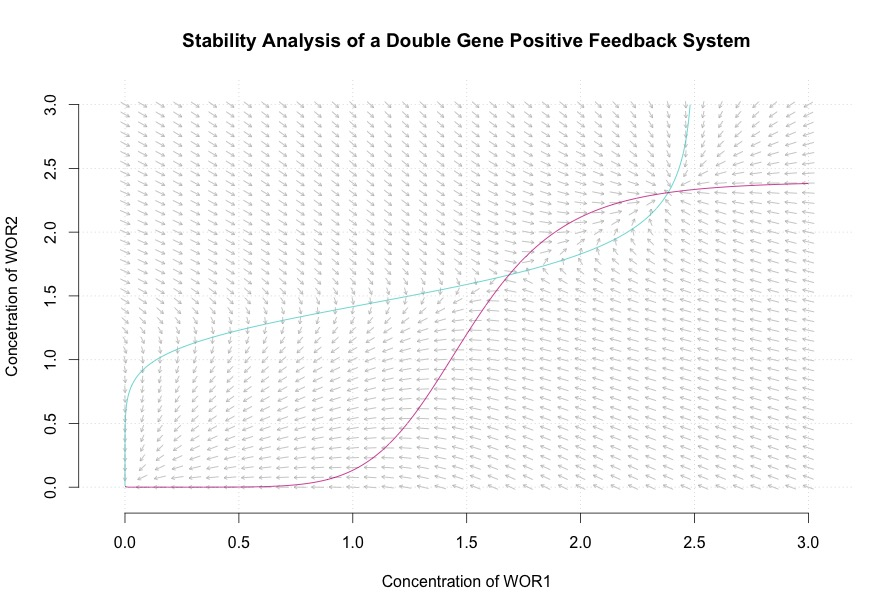
\includegraphics[width=0.6\textwidth]{./figures/stabilityDoublePositive.jpeg}
            \caption{The stability of stationary point present in a double gene positive feedback system. The red line represents the nullcline for the protein and blue the nullcline of mRNA. The arrows represent the direction of change for the system at a given state.}
            \label{stabilityDoublePositive}
            \end{figure}
            
            \subsubsection{Negative Feedback}
            Although, a known double feedback does not directly exist between two genes in Candida Albicans it is perhaps the most interesting situation to look at. The system is depicted in Figure \ref{doubleNegative}, and the equation describing it are identical to those describing the positive apart from the negative hall equation being used as described in the negative single gene model. Again, applying our standard analysis for stability of the system Figure \ref{stabilityDoubleNegative} we see something completely different to the single gene case. Whereas the single gene with negative feedback only produce a single stationary and stability point the double gene with mutual negative feedback generates three stationary point with two of them being stable. This demonstrates that you can generate a bistable system out of solely negative feedback. An indirect double negative feedback system exists in Candida Albicans but requires the modelling of an additional gene which is beyond the scope of this paper.
            
            \begin{figure}[h]
            \centering
            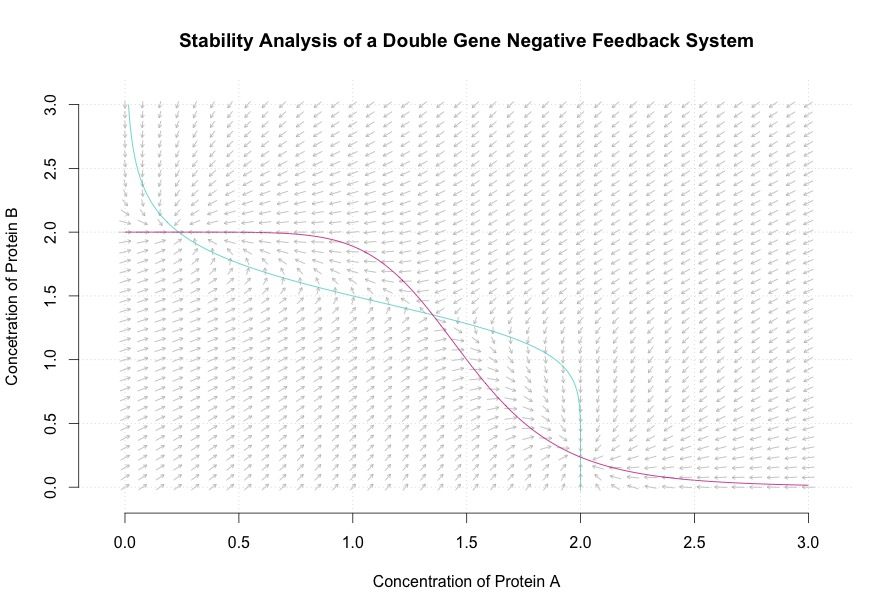
\includegraphics[width=0.6\textwidth]{./figures/stabilityDoubleNegative.jpeg}
            \caption{The stability of stationary point present in a double gene negative feedback system. The red line represents the nullcline for the protein and blue the nullcline of mRNA. The arrows represent the direction of change for the system at a given state.}
            \label{stabilityDoubleNegative}
            \end{figure}
 

            \begin{figure}[h]
            \centering
            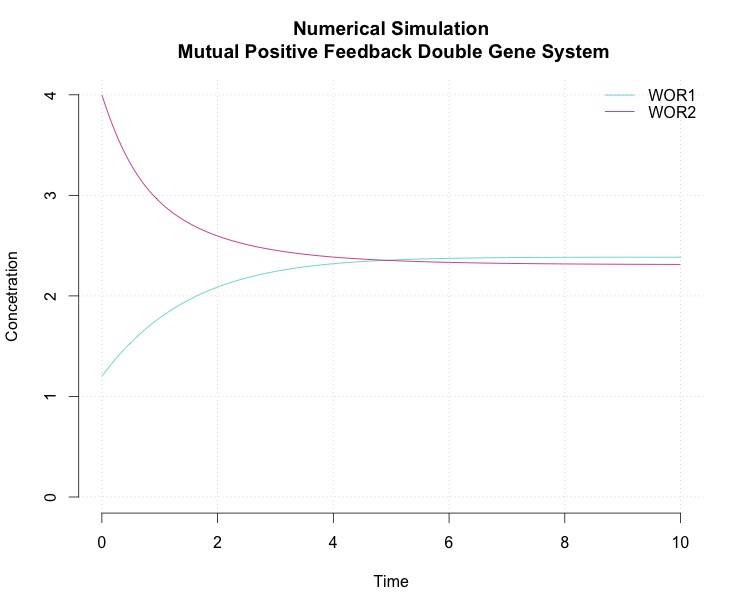
\includegraphics[width=0.6\textwidth]{./figures/simDoublePos.jpeg}
            \caption{A numerical simulation of a double gene positive feedback system.}
            \label{simDoublePos}
            \end{figure}

\bibliographystyle{unsrt}
\bibliography{Bibliography}

\end{document}